\begin{figure}[htbp]
\centering
\(\displaystyle
 0 \xrightarrow[\text{order }2]{\,c_4T_2\,} -c_4
   \xrightarrow[\text{order }1]{\,T_8\,} 0,
 \qquad
 P_4=T_8\circ(c_4T_2),\quad c_4=\cos(\pi/16)
\)\par\medskip
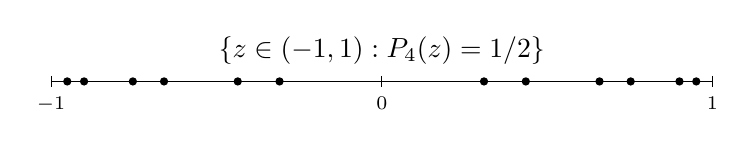
\begin{tikzpicture}[x=4.2cm,y=1cm]
 \draw[semithick] (-1,0)--(1,0);
 \foreach \x in {-1,0,1}{
    \draw (\x,.07)--(\x,-.07) node[below,font=\scriptsize] {\(\x\)};
 }
 \foreach \a in {5,7,11,13,17,19}{
   \pgfmathsetmacro{\xx}{sqrt((1+cos(7.5*\a)/cos(11.25))/2)}
   \fill (\xx,0) circle[radius=1.5pt];
   \fill (-\xx,0) circle[radius=1.5pt];
 }
 \node[above] at (0,.09) {\(\{z\in(-1,1):P_4(z)=1/2\}\)};
\end{tikzpicture}
\caption{The first vertical return block \(P_4=T_8\circ(c_4T_2)\). Top: the critical point \(0\) returns to \(0\) with local order two. Bottom: the regular value \(1/2\) has twelve simple inverse images in \((-1,1)\), giving distinct local inverse charts for the fold.}
\label{fig:fold-block}
\end{figure}
